\section{Introduction}

The technological advancements in recent decades lead to more intensive experiments in Nuclear Physics. The experiments are conducted with higher luminosities (higher frequency of beam to target interactions), and more complex detector systems with many more channels. This leads to increased data rates originating from each individual detector component. As a result, the data volume has significantly increased compared to the past experiments. The increased data volume presents challenges in data transfer and persistence, requiring more storage facilities. There are known methods for compressing the experimental raw data using lossless compression algorithms that can reduce the stored data size. However, the lossless compression methods are usually slow and are not suitable for the online data acquisition stage, since they do not provide sufficient throughput. 
New advances in neural networks have had a significant impact on the field of nuclear physics. Neural networks can be used to solve a variety of problems in nuclear physics, including simulation of nuclear reactions, data analysis, reconstruction of events from detector data, and many more. The use of neural networks in nuclear physics is still in its early stages, but it has the potential to revolutionize the field. As neural networks become more powerful and sophisticated, they will be able to solve even more problems in nuclear physics.

In this paper, we investigate Machine Learning (ML) methods for lossy raw data compression and their applications in online data acquisition.

\section{CLAS12 Detector}

The CLAS12 detector, located in experimental Hall-B at Jefferson lab, is designed 
to study electro-induced nuclear and hadronic reactions by providing efficient 
detection of charged and neutral particles over a large fraction of the full solid angle. 
The detector is based on a combination of a six-coil torus magnet and
a high-field solenoid magnet. The combined magnetic field provides a large 
coverage in both azimuthal and polar angles; a schematic view is presented in Figure~\ref{fig:CLAS12}. 

\begin{figure}[h!]
\centering
%\centerline{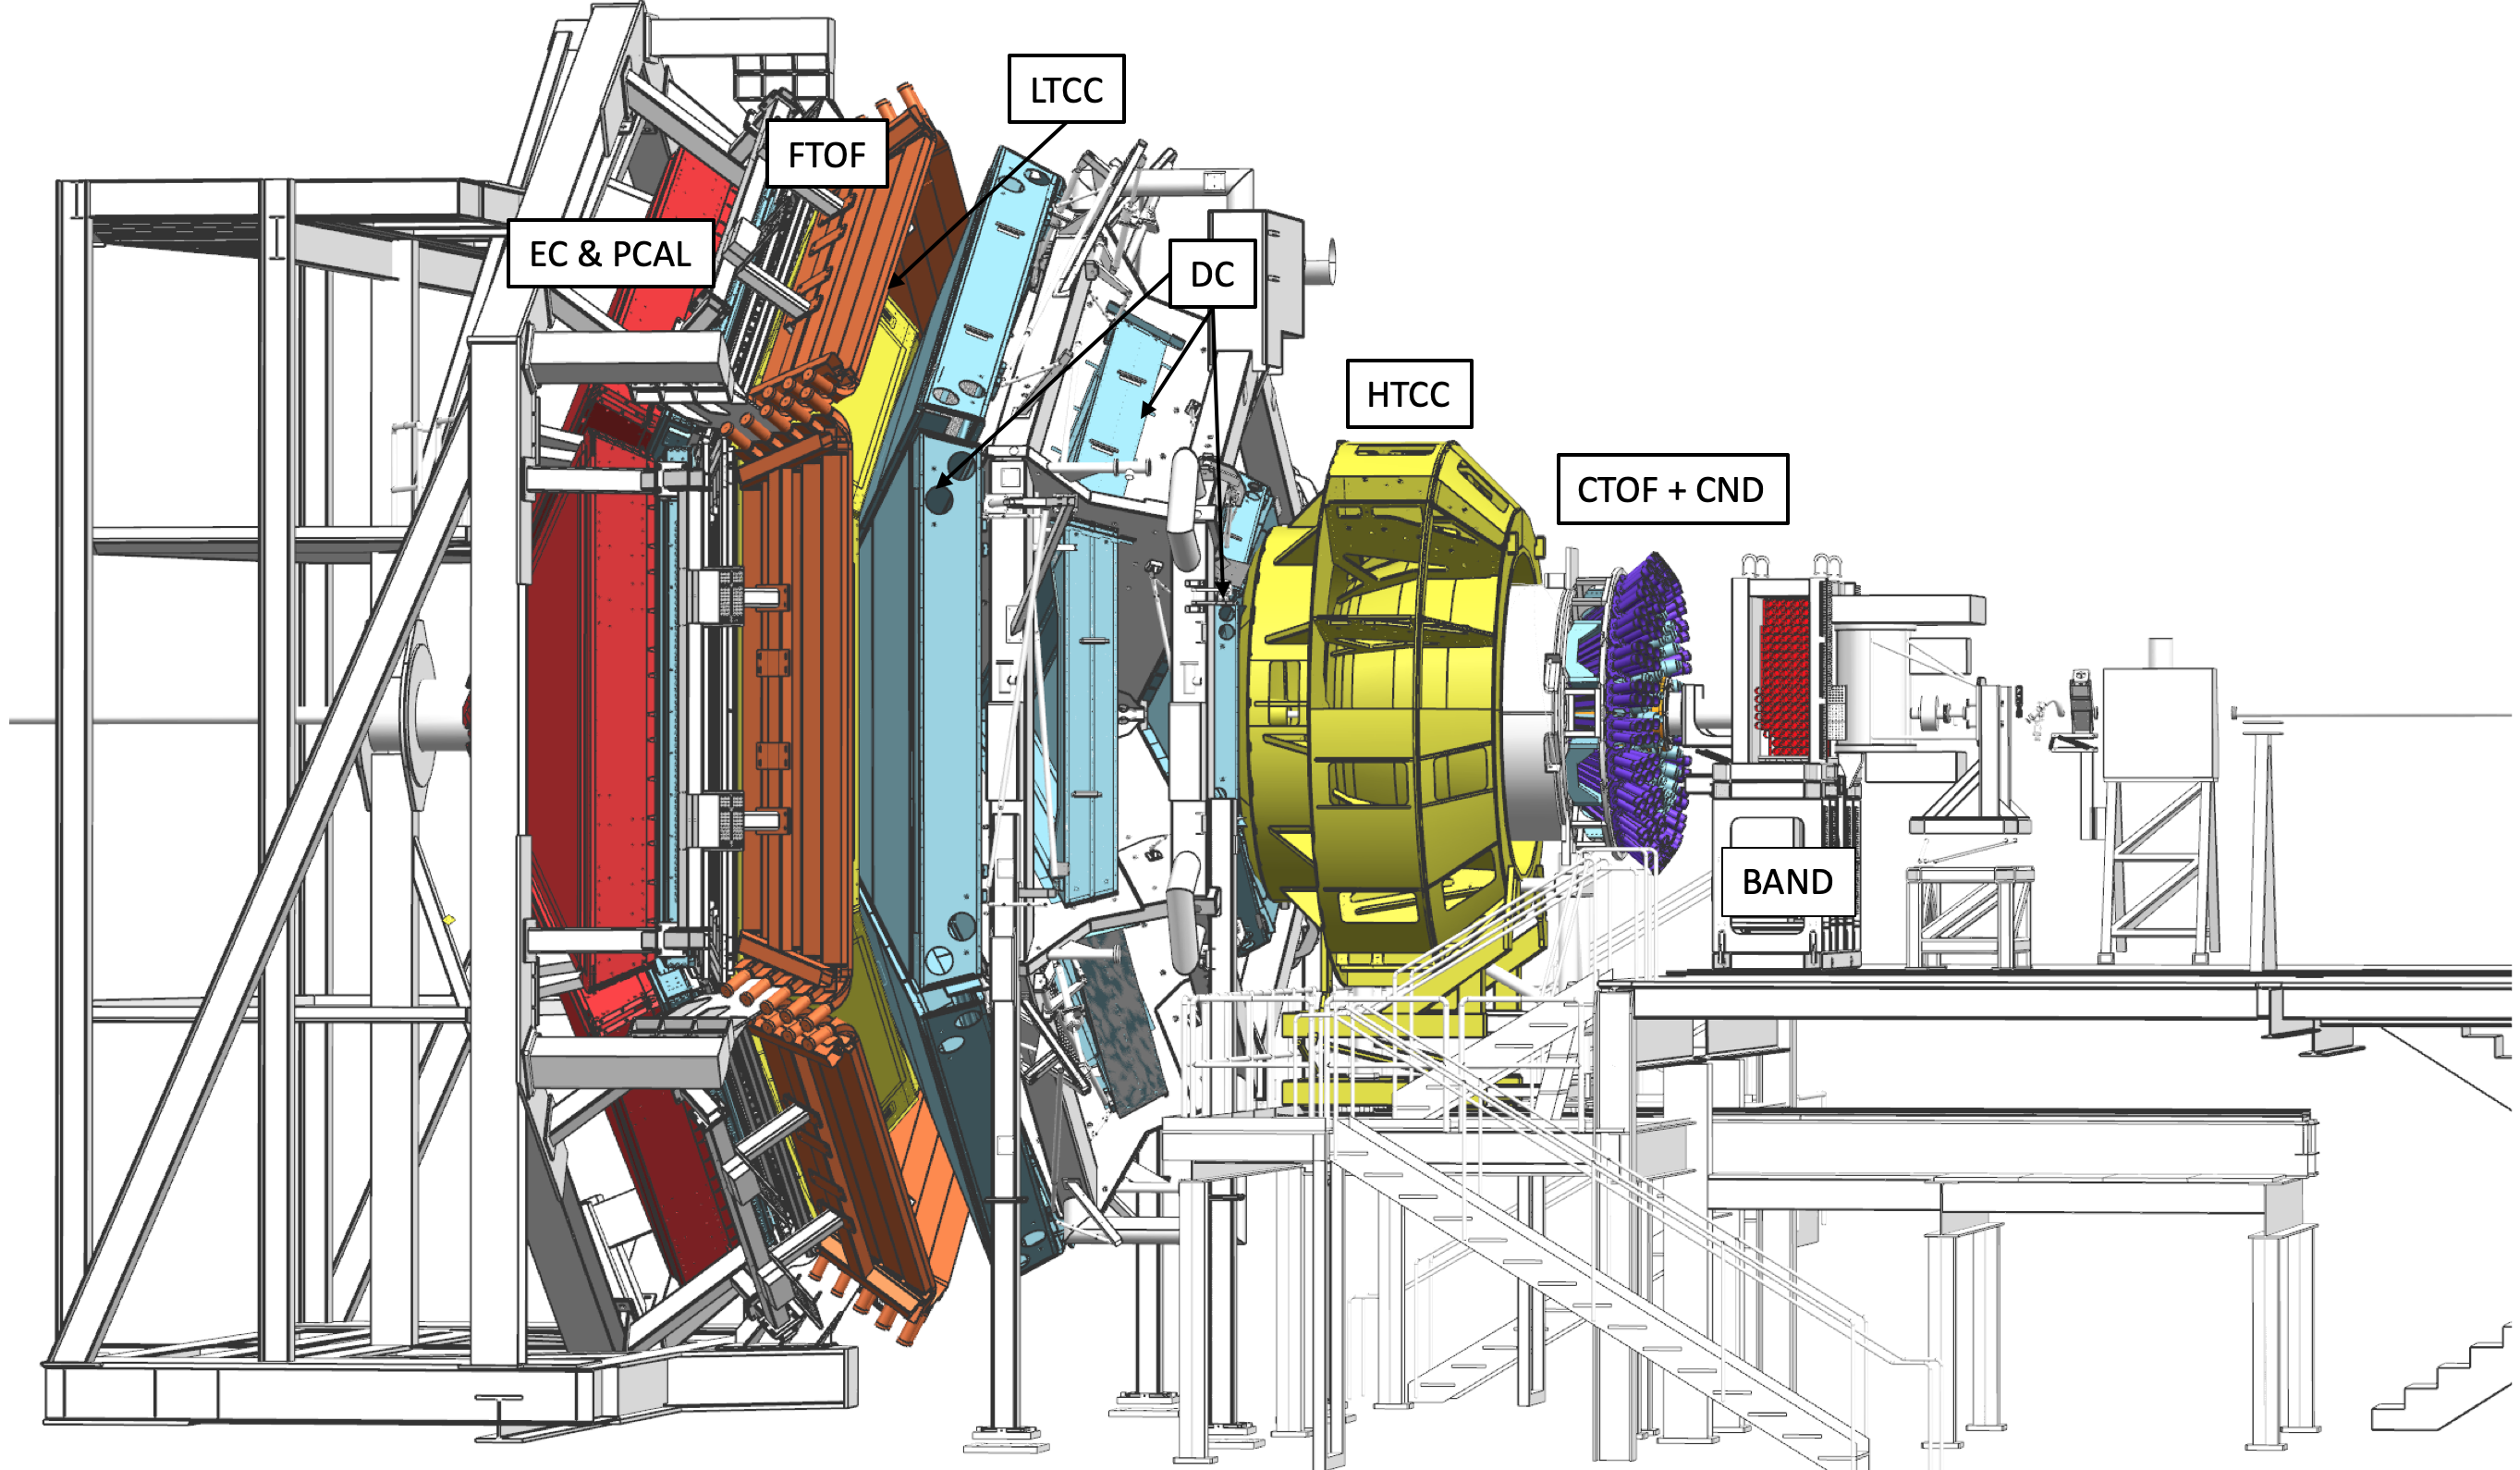
\includegraphics[width=0.7\columnwidth]{CLAS12-side.png}}
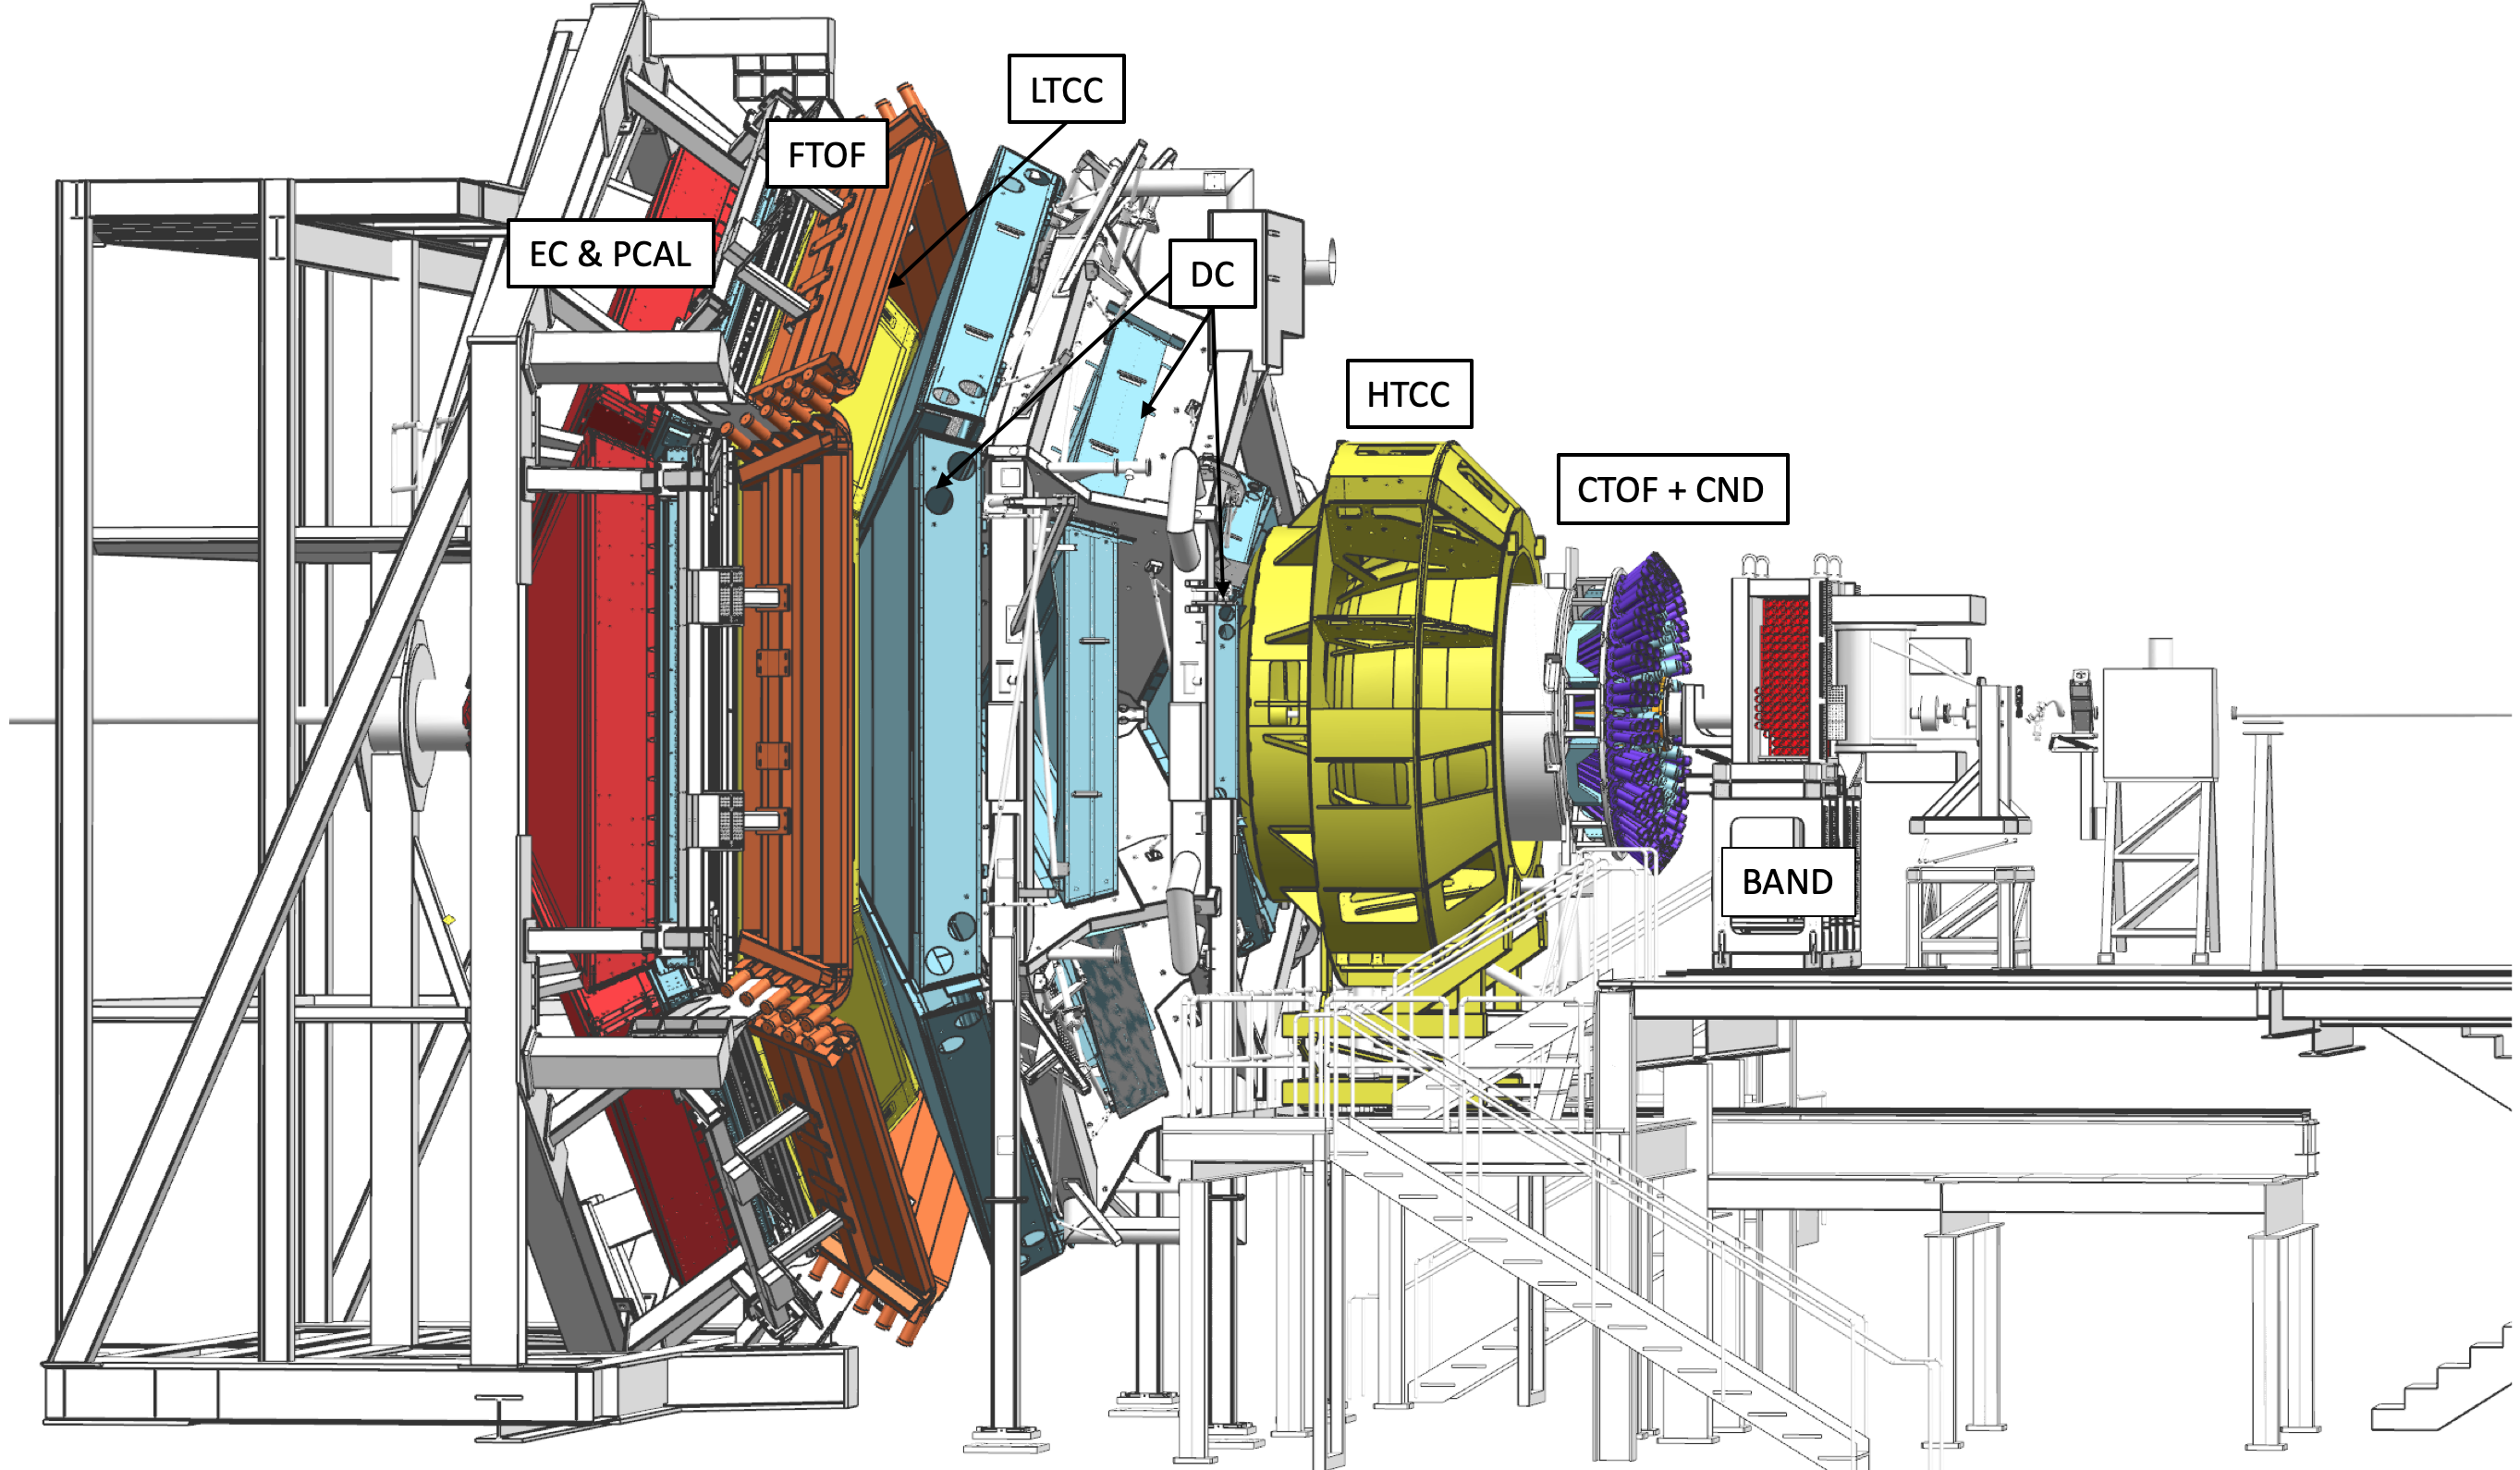
\includegraphics[width=0.7\columnwidth]{CLAS12-side.png}
\caption{The CLAS12 detector in the Hall~B beamline ~\cite{Burkert:2020akg}. The electron beam enters from the right and impinges on
  the production target located in the center of the solenoid magnet shown at the right (upstream) end of CLAS12,
  where other detector components are also visible. Scattered electrons and forward-going particles are detected
  in the Forward Detector (FD), consisting of the High Threshold Cherenkov Counter (HTCC) (yellow), 
  %with full coverage in polar angle $5^\circ \le \theta \le 35^\circ$ and $\Delta \phi = 2\pi$ coverage in azimuth. The HTCC is followed
  followed by the torus magnet (gray), the drift chamber tracking system (light blue),
  and time-of-flight scintillation counters (brown), and electromagnetic calorimeters (red). 
  %Between the HTCC and the
  %torus, the Forward Tagger is installed to detect electrons and photons at polar angles $2^\circ \le \theta \le 5^\circ$.
  %The Central Detector (CD) consists of the Silicon Vertex Tracker (hidden), which is surrounded by a Barrel Micromesh
  %Tracker (hidden), the Central Time-of-Flight system, and the Central Neutron Detector (PMTs in blue). At the upstream
  %end, a Back Angle Neutron Detector (red) is installed. In the operational configuration. the entire CLAS12 detector
  %extends for 13~m along the beamline.
  } 
\label{fig:CLAS12}
\end{figure}

Some of CLAS12 detector components (such as Time-Of-Flight counters and Electromagnetic Calorimeters) have an FADC readout which is measuring the charge in $4~ns$ intervals. The measured pulses are used in reconstruction to calculate the pulse integral charge and time. The charge integral is used to determine the deposited energy in the detector component such as individual calorimeter scintillating paddles. Having an entire pulse spectrum provides more accuracy in deposited energy measurement since the pedestal subtracted pulse can be obtained from the pulse shape and fitted. The pulse shape also provides timing information which helps in combining hits into clusters. Example pulses from the electormagnetic calorimeter can be seen in Figure~\ref{fig:pulse_examples}.
\begin{figure}[h!]
\centering
%\centerline{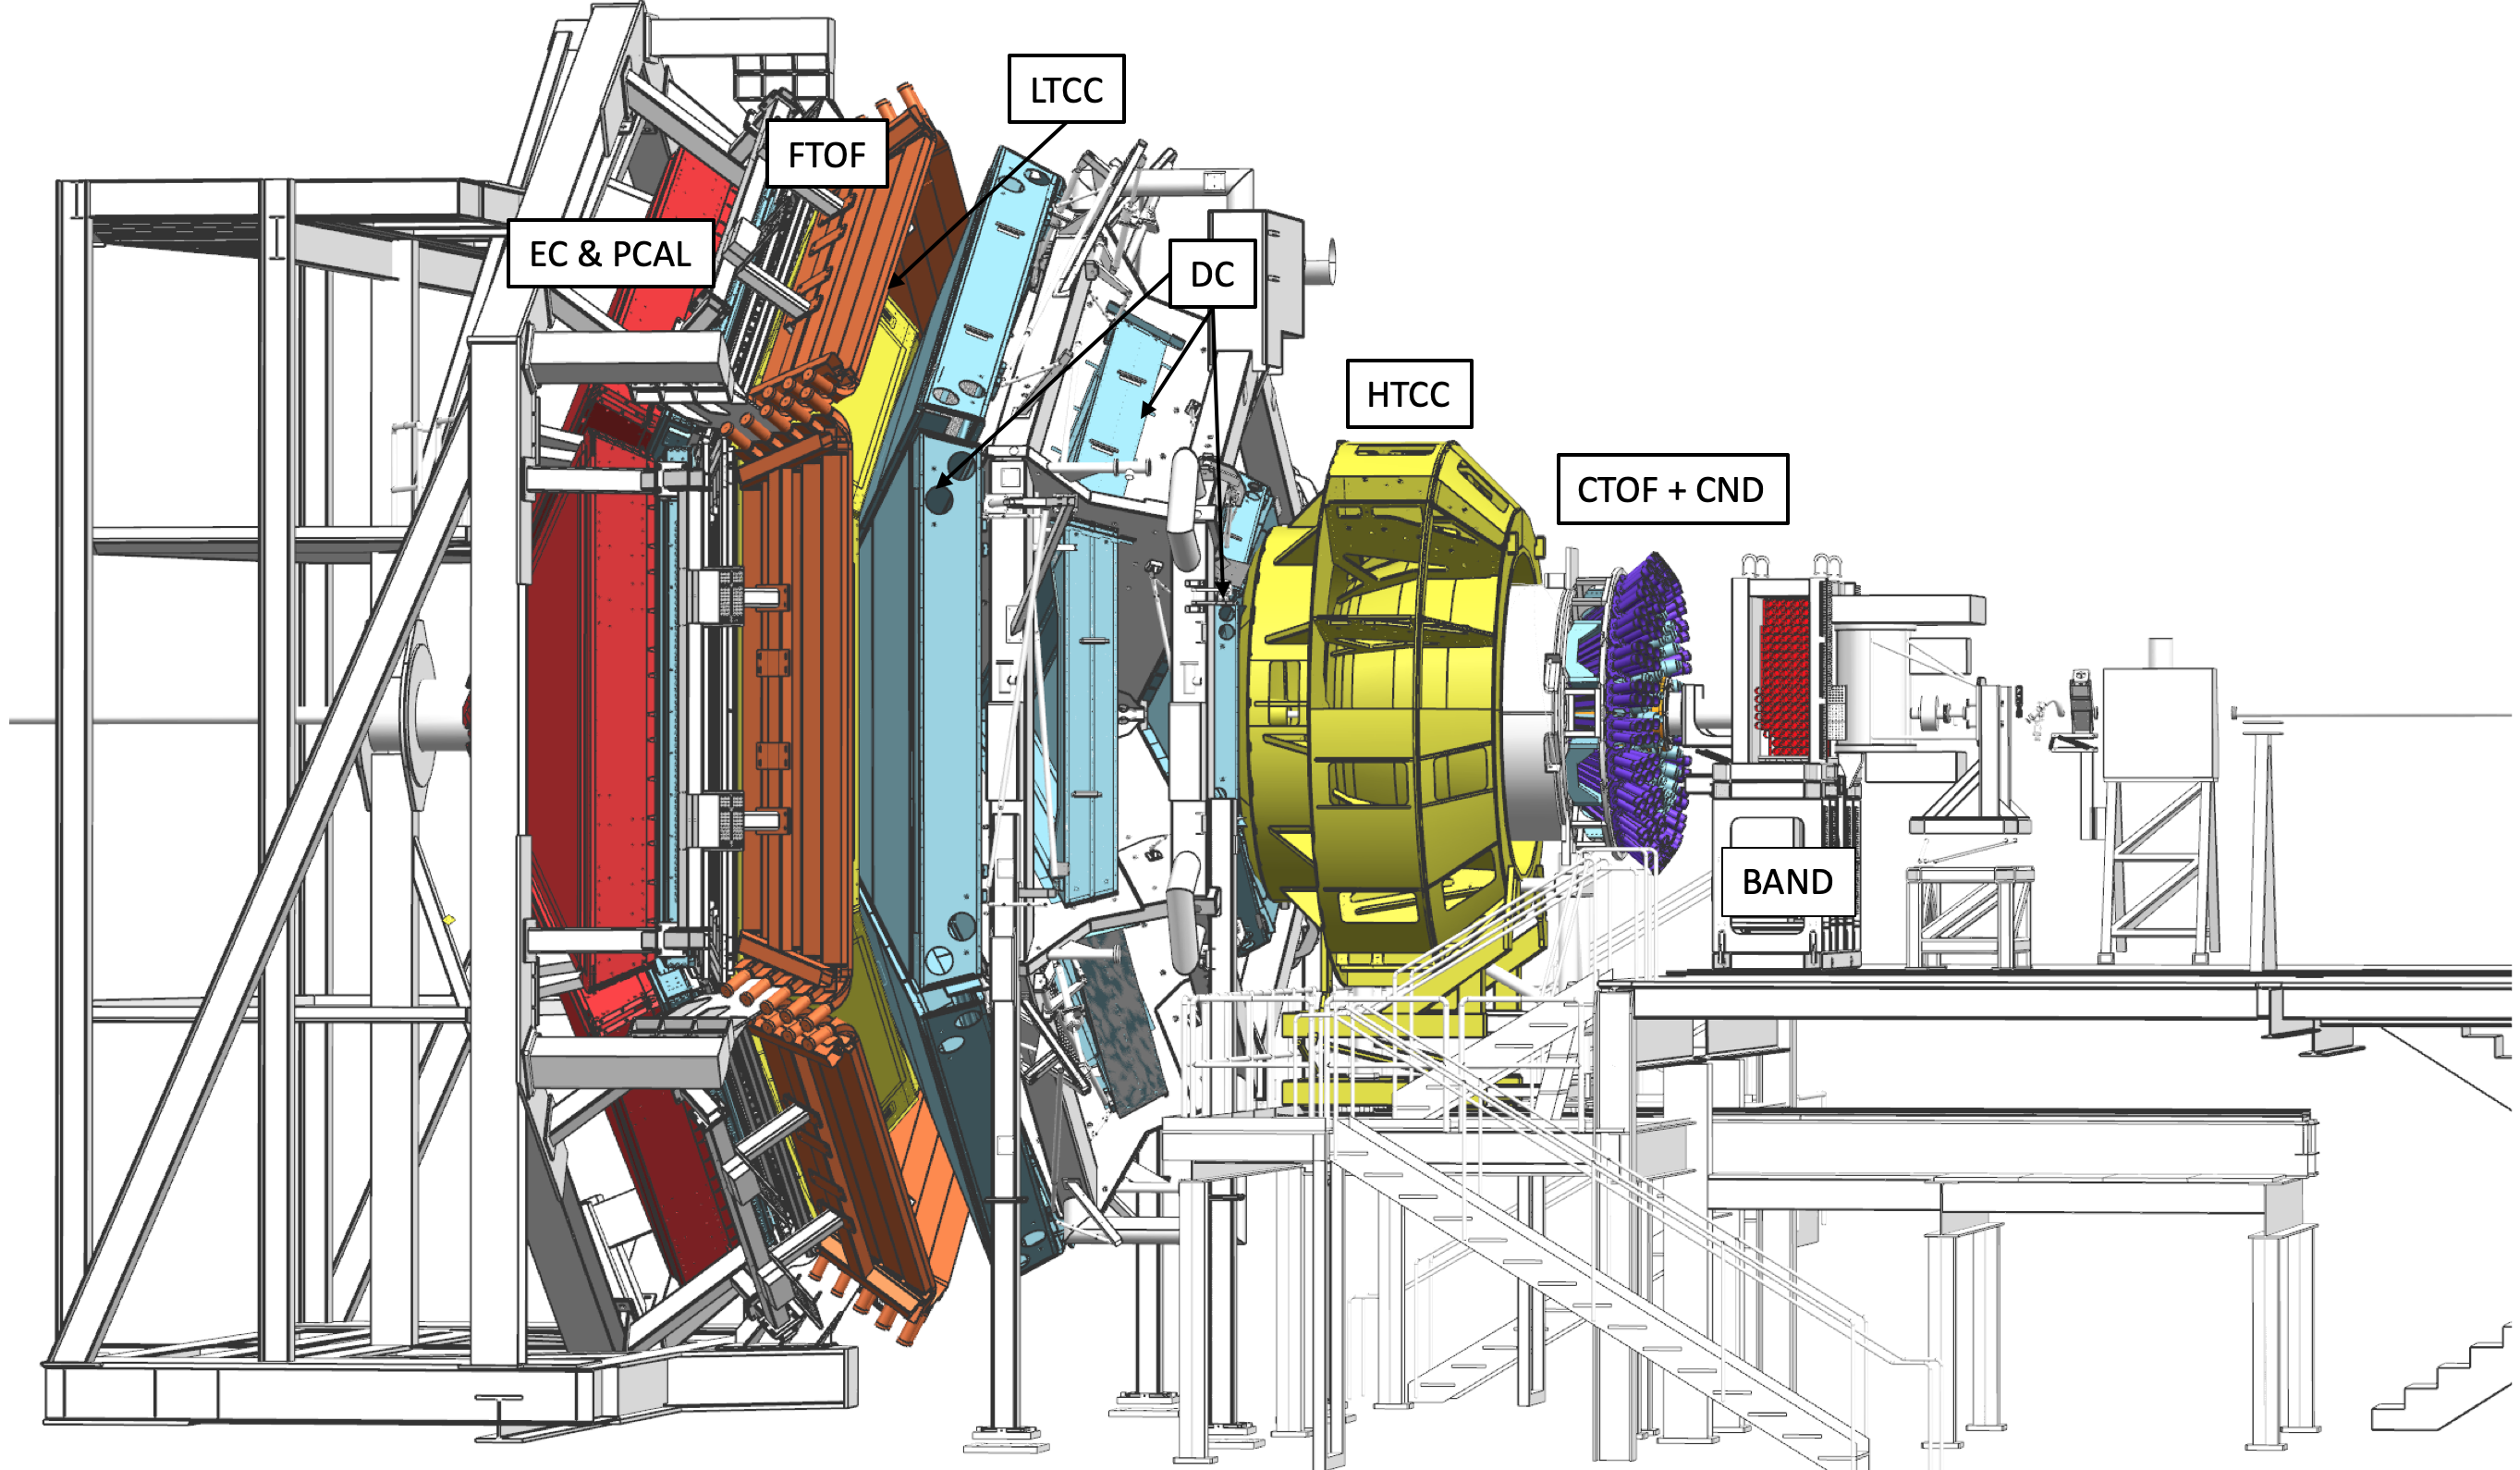
\includegraphics[width=0.7\columnwidth]{CLAS12-side.png}}
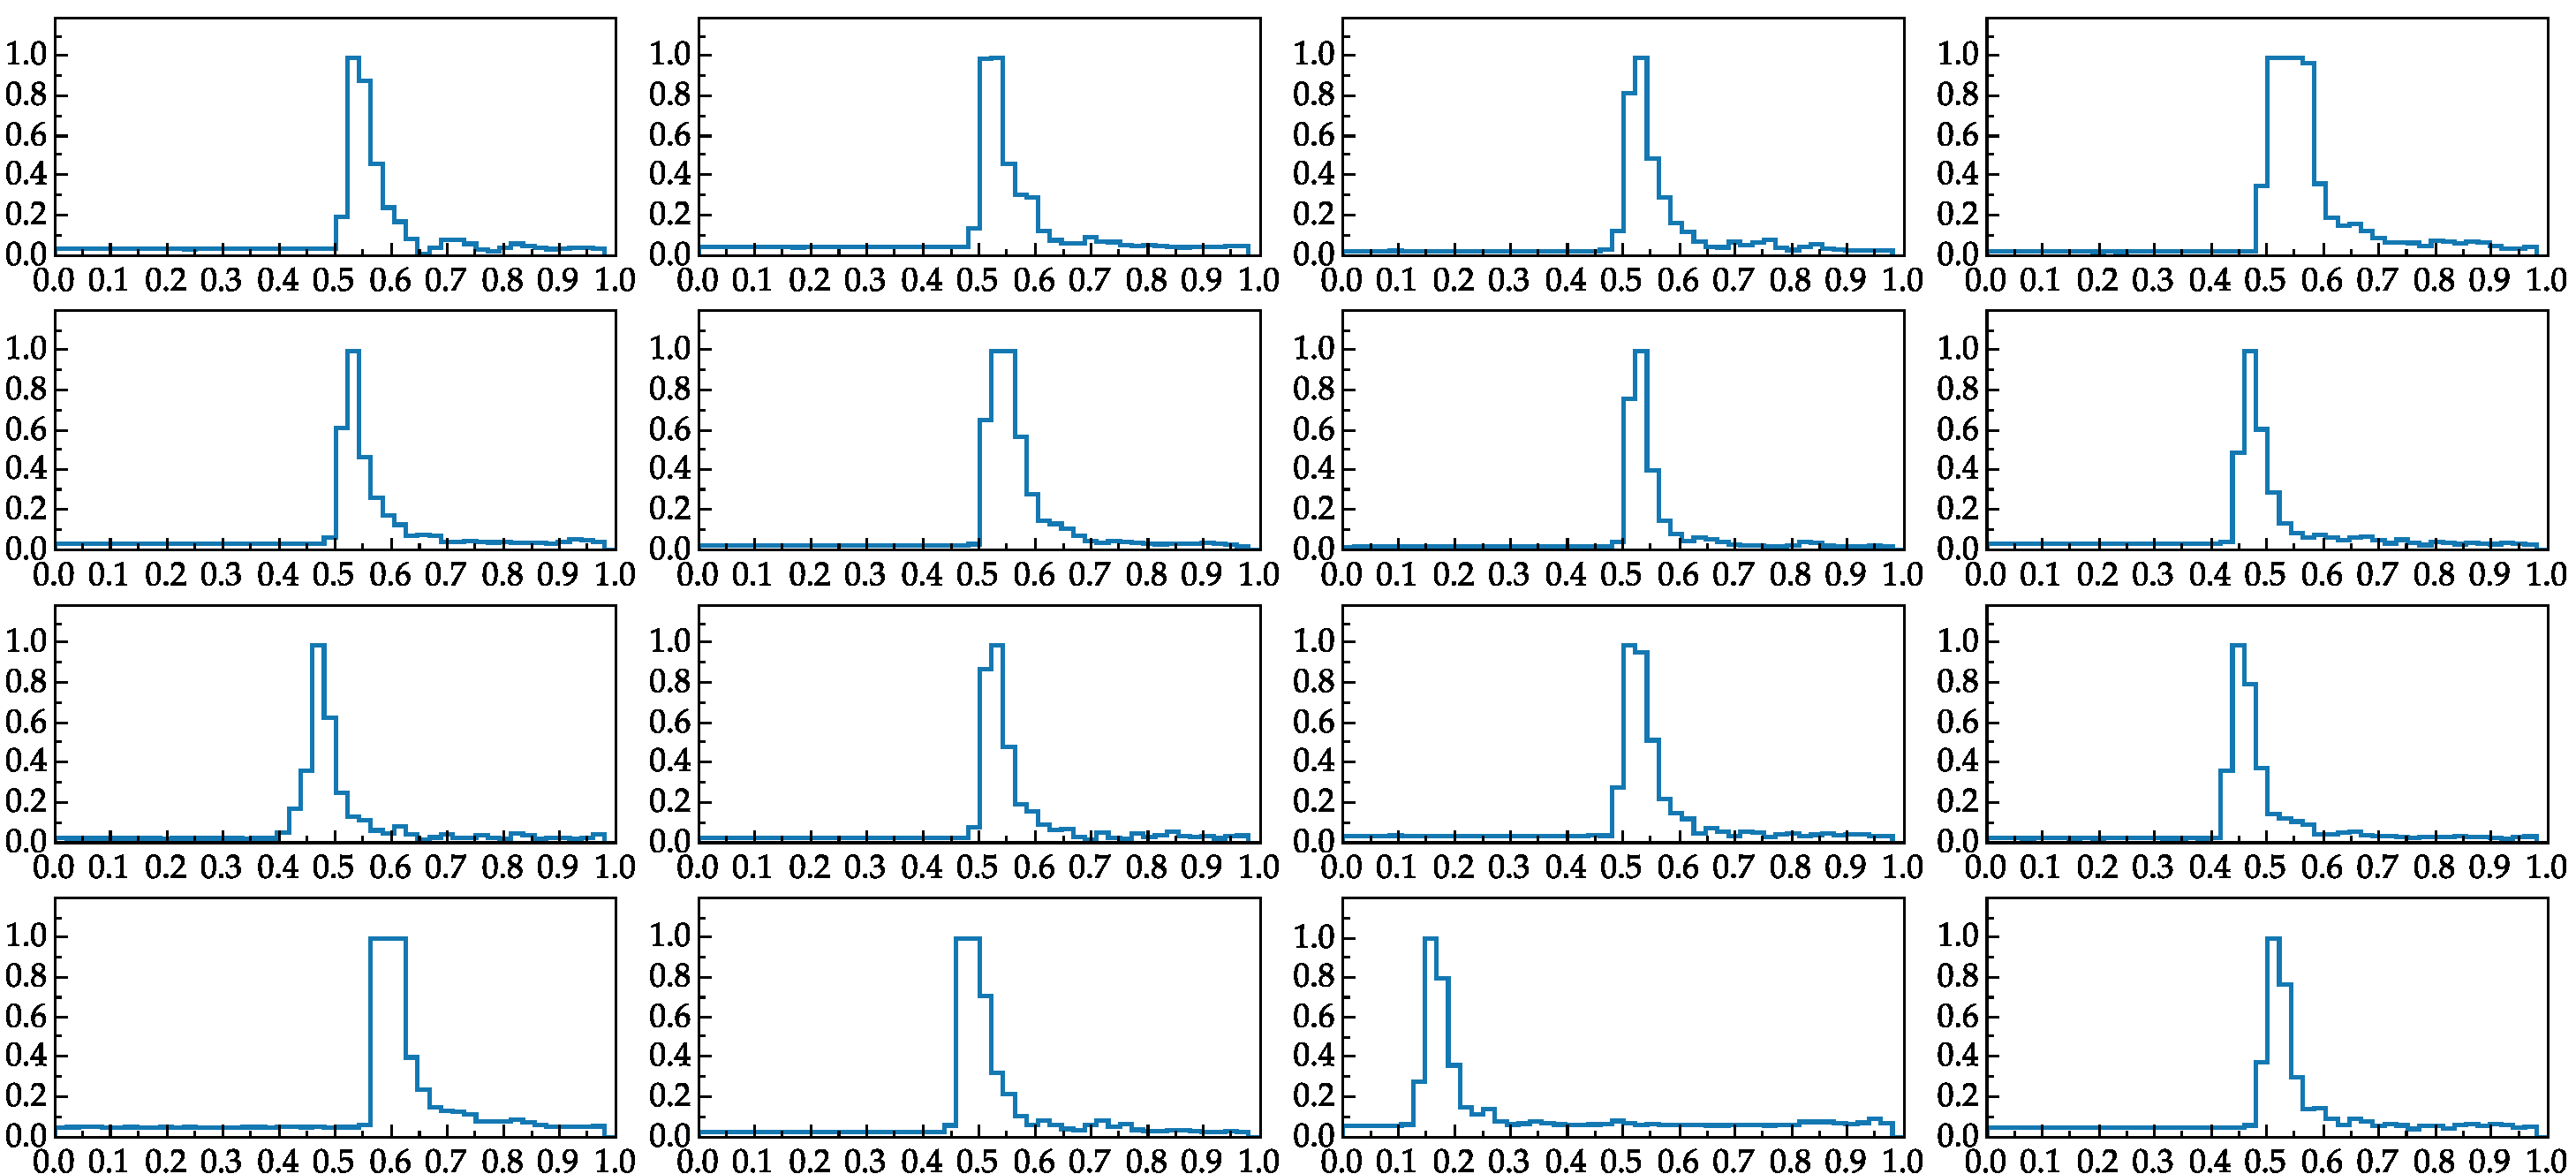
\includegraphics[width=0.9\columnwidth]{ec_pulse_examples.pdf}
\caption{ Example pulses from Electromagnetic Calorimeter (EC) of CLAS12 detector. (The pulses are normalized to the peak height)}
\label{fig:pulse_examples}
\end{figure}
However, the accuracy comes at a cost of data size, because instead of keeping one value of integrated charge (one floating number of 4 bytes) the pulse profile is stored in the output data stream consisting of 48 short numbers (96 bytes). 

